%%%%%%%初期設定 start%%%%%%%%%%%%%%%%%%%%%%%%%%%%%%%%%%%%%%%%%%%%%

\documentclass[12pt]{jsreport}%pLaTeX対応
\renewcommand{\bibname}{参考文献} 
\usepackage[dvipdfmx]{graphicx}
\usepackage{ascmac, url, array, ./style/eclbkbox}

\setlength{\textheight}{25cm}		%1ページ当りの行数を指定する
\setlength{\textwidth}{38zw}		%1行あたりの文字数の設定
\setlength{\evensidemargin}{10mm}   %偶数ページの余白
\setlength{\oddsidemargin}{10mm}    %奇数ページの余白
\setlength{\topmargin}{-3mm}        %上の余白
\setlength{\headheight}{0mm}        %ヘッダ領域の高さ


\setlength{\headsep}{0mm}           %ヘッダ領域と本文領域との間隔
\setlength{\columnsep}{12mm}        %段組にした場合の段同士の間隔
\setlength{\footskip}{10mm}         %フッタ領域と本文との間隔

%%%%%%%タイトル内容 start%%%%%%%%%%%%%%%%%%%%%%%%%%%%%%%%%%%%%%%%%%

\title{FaceAPIを用いた表情分析を活用した労務管理支援の提案}					%卒業論文タイトル
\author{1132115 中村 香菜\\1232XXX 工大 太郎\\\normalsize 指導教員:中村 直人 教授}	%名前(苗字と名前は全角1字空け)
\date{平成27年度}                                %日付設定(デフォルトは現在の年月日)

%%%%%%%タイトル内容 end%%%%%%%%%%%%%%%%%%%%%%%%%%%%%%%%%%%%%%%%%%%

%%%%%%%初期設定 end%%%%%%%%%%%%%%%%%%%%%%%%%%%%%%%%%%%%%%%%%%%%%

%%%%%%%コンテンツ start%%%%%%%%%%%%%%%%%%%%%%%%%%%%%%%%%%%%%%%%%%%%
\begin{document}
\pagenumbering{roman}
\maketitle                          %タイトルをドキュメントへ貼り付け
\tableofcontents                 %目次を作成
\listoffigures				 %図の目次作成
\listoftables				 %表の目次作成

\baselineskip 20pt               %行間設定


\clearpage
\pagenumbering{arabic}

%%%%%%%本文 start%%%%%%%%%%%%%%%%%%%%%%%%%%%%%%%%%%%%%%%%%%%

%別ファイルを読み込み
%\input{ディレクトリ名/ファイル名}
%http://www.latex-cmd.com/
\chapter{はじめに}
\label {chp:tex_basic}

\section{研究の背景と目的}
\label{sec:tex_basic_section}
昨今,コロナの影響により,人と直接会う機会が減り,マスクの着用を強いられるようになった.
その結果,笑顔になる機会が減るため,笑顔の減少に繋がる.
しかし,総合人材サービスのパーソルホールディングス株式会社が行った調査[1]では,
仕事をする上で笑顔になると「楽しい」という気持ちが高まった人は約6割で,
ポジティブな感情状態で仕事に取り組んでいた人ほど,笑顔になっており,
職場において笑顔が高まれば,自発的に取り組む傾向があるという結果が出た.

\begin{figure}[!h]
    \begin{center}
        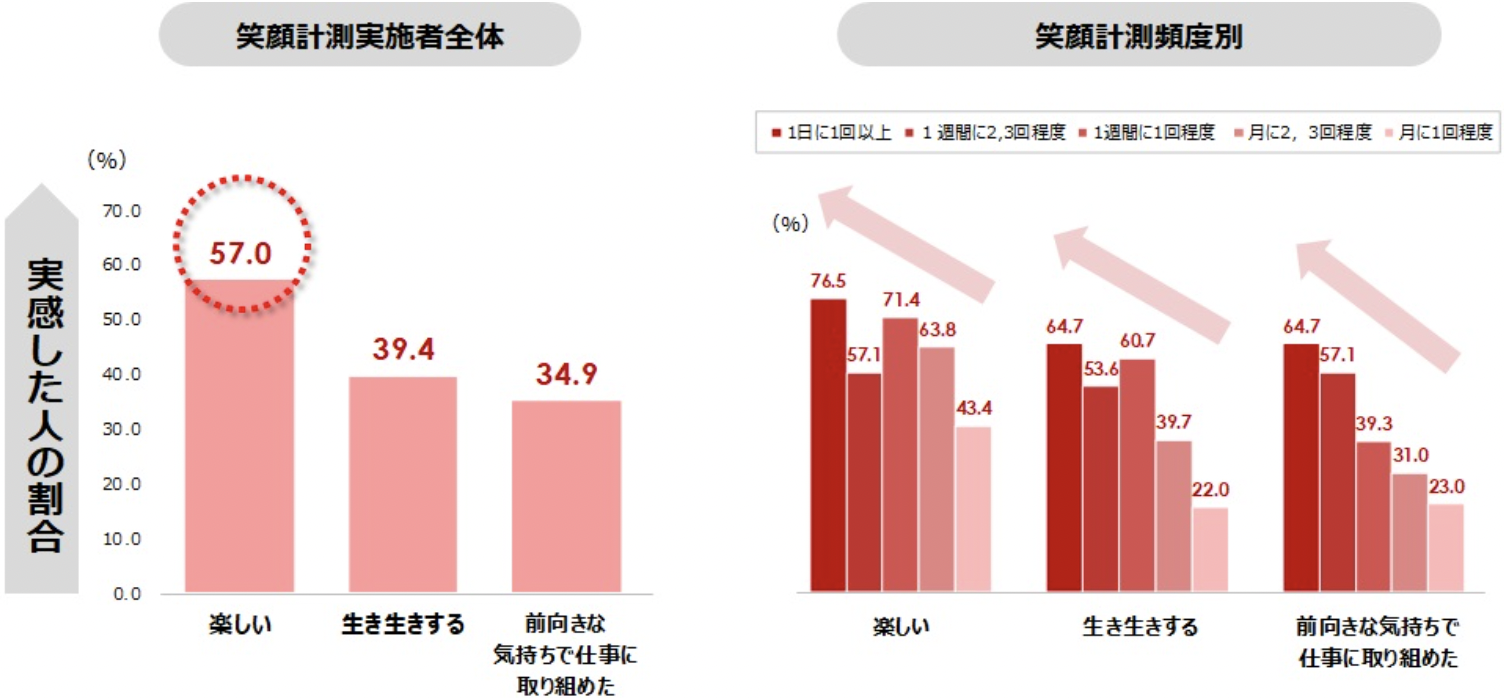
\includegraphics[scale=0.5, clip]{./img/work.png}
        \caption{笑顔計測後の主な感情変化}
        \label{fig:図の名前}
    \end{center}
\end{figure}

また,厚生労働省の調査[2]によると,下のグラフから分かるように,厚生労働省の調査によると,
平成19年度から令和元年にかけて約15\%も増加している.

\begin{figure}[!h]
    \begin{center}
        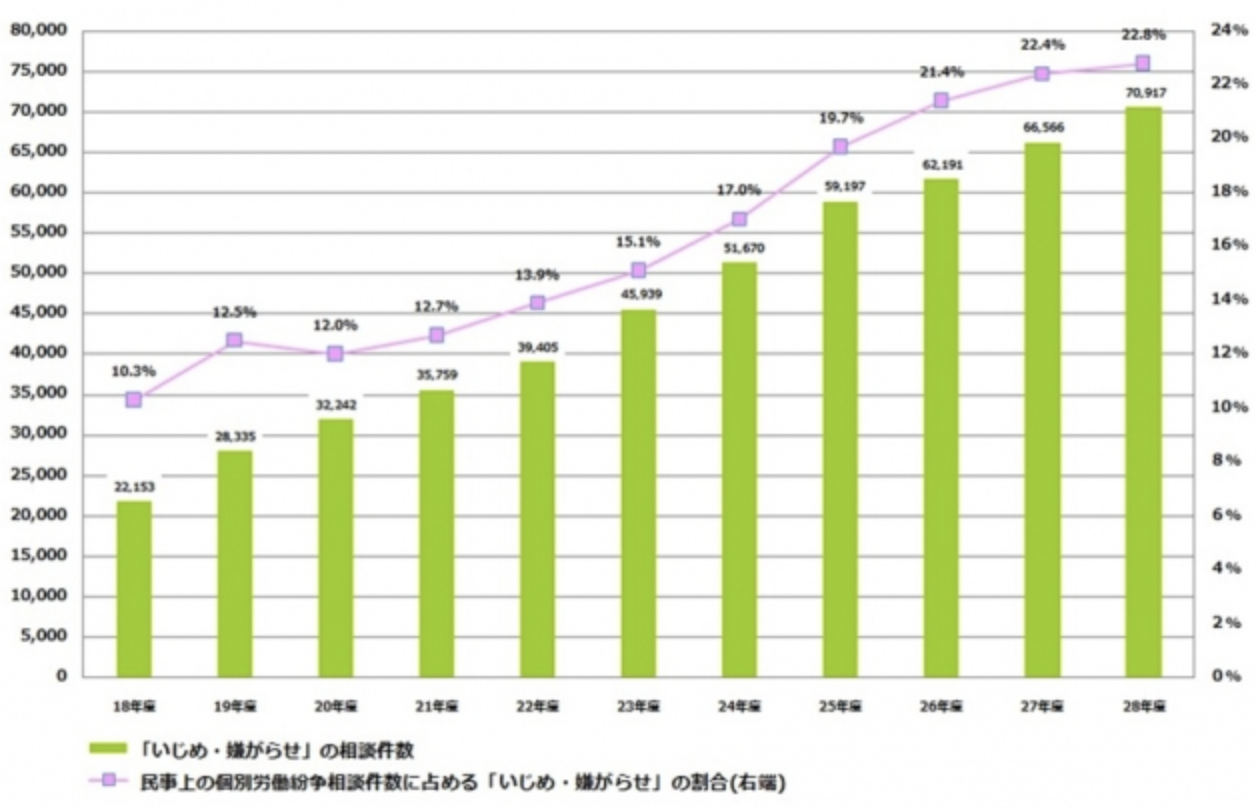
\includegraphics[scale=0.6, clip]{./img/graph.png}
        \caption{厚生労働省によるパワハラ調査}
        \label{fig:図の名前}
    \end{center}
\end{figure}

そこで我々は,以上の課題である「笑顔の減少」と「パワハラの増加」の解決を目的に
FaceAPIを用いた表情分析を活用した労務管理支援システムを提案する.

\vspace{8mm}

\section{論文の構成}
\label{sec:tex_basic_newline}
    改行は\verb|\\|というように,バックスラッシュ(円マーク)を続けて二つ記述します.\\
    \%を書くと以降がコメントアウトされます.

    エディタ上で一行空白をあけて記述することで,新たな文節として認識されます.

\section{環境とコマンド}
\label{sec:tex_basic_envcmd}
    Latexには「環境」と「コマンド」があります.
    環境は複数行にまたがるもので,コマンドは一行のみ有効なものです.
\subsection{環境}
\label{sub:tex_basic_section_envcmd_env}
    環境を使用するときは\verb|\begin{環境名}と\end{環境名}|で囲みます.\\
    画像を表示,表を作成,箇条書き等さまざまな場面で使用します.
\subsection{コマンド}
\label{sub:tex_basic_section_envcmd_cmd}
    コマンドは\verb|\newpage|のように先頭に\verb|\|をつけた単語を記述します.\\
    環境と同様にさまざまな種類があります.

\section{エスケープ}
\label{sec:tex_basic_escape}
    \# \$ \& \% \{ \}  \\
    などがエスケープの必要な文字です.直前に\verb|\|をつけるとエスケープされます.\\
    文章全体をエスケープする場合は「verbatim」環境を使用します.
     
\section{箇条書き}
\label{sec:tex_basic_clause}
    箇条書きを行う場合にはitemize環境を使用します.\\
    改行を入れることで題目と説明のように表示することが可能です.\\
    |記述例|\\
    \verb|\begin{itemize}|\\
        \verb|\item| あいてむ1\\
        \verb|\item| あいてむ2\\\\
        あいてむ2について\\
    \verb|\end{itemize}|\\\\
    |表示例|
\begin{itemize}
    \item あいてむ1
    \item あいてむ2

    あいてむ2についてあいてむ2についてあいてむ2についてあいてむ2についてあいてむ2についてあいてむ2についてあいてむ2についてあいてむ2についてあいてむ2についてあいてむ2についてあいてむ2についてあいてむ2についてあいてむ2についてあいてむ2についてあいてむ2について
\end{itemize} 

    箇条書きには複数種類があります.\\
    itemize環境の場合は通常の「・」,enumerate環境の場合は「1.」のように数字列挙に,description環境の場合は「\verb|\item[項目A] 説明文|」と書くことで項目つきの箇条になります.

\chapter{図表の挿入}
\label{chp:chart}

\section{図の表示}
\label{sec:chart_figure}
    図を表示する場合,figure環境を使用します.画像はpng、jpg、pdfが使用できます.\\

    |記述例:PNG|
    \begin{verbatim}
    \begin{figure}[!h]
    \begin{screen}
    \begin{center}
        
\includegraphics[scale=0.4, clip]{./img/apple.png}    
        \caption{図の名前}
        \label{fig:図の名前}
    \end{center}
    \end{screen}
    \end{figure}
    \end{verbatim}

    |表示例:PNG|
    \begin{figure}[!h]
    \begin{screen}
    \begin{center}
        
\includegraphics[scale=0.4, clip]{./img/apple.png}
        \caption{図の名前}
        \label{fig:図の名前}
    \end{center}
    \end{screen}
    \end{figure}

    |記述例:JPG|
    \begin{verbatim}
    \begin{figure}[!h]
    \begin{screen}
    \begin{center}
        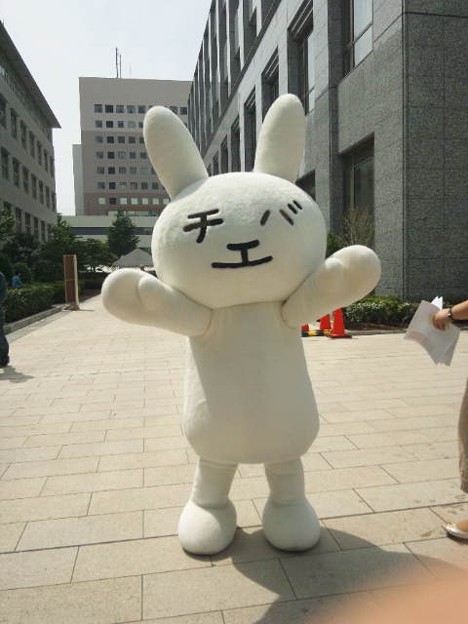
\includegraphics[scale=0.4, clip]{./img/CIT.jpg}    
        \caption{図の名前}
        \label{fig:図の名前}
    \end{center}
    \end{screen}
    \end{figure}
    \end{verbatim}

    |表示例:|
    \begin{figure}[!h]
    \begin{screen}
    \begin{center}
        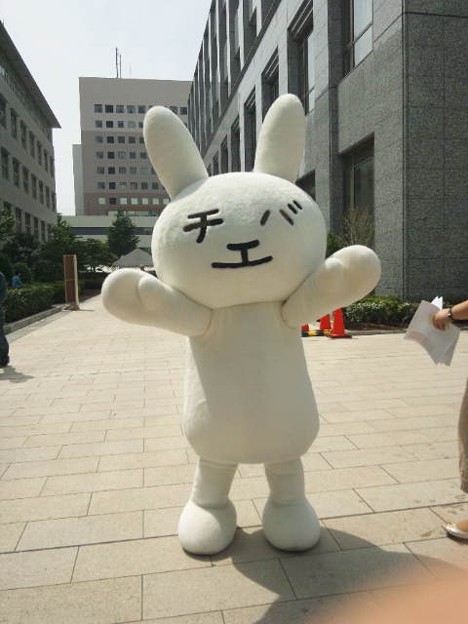
\includegraphics[scale=0.4, clip]{./img/CIT.jpg}
        \caption{図の名前}
        \label{fig:図の名前}
    \end{center}
    \end{screen}
    \end{figure}

    |記述例:PDF|
    \begin{verbatim}
    \begin{figure}[!h]
    \begin{screen}
    \begin{center}
        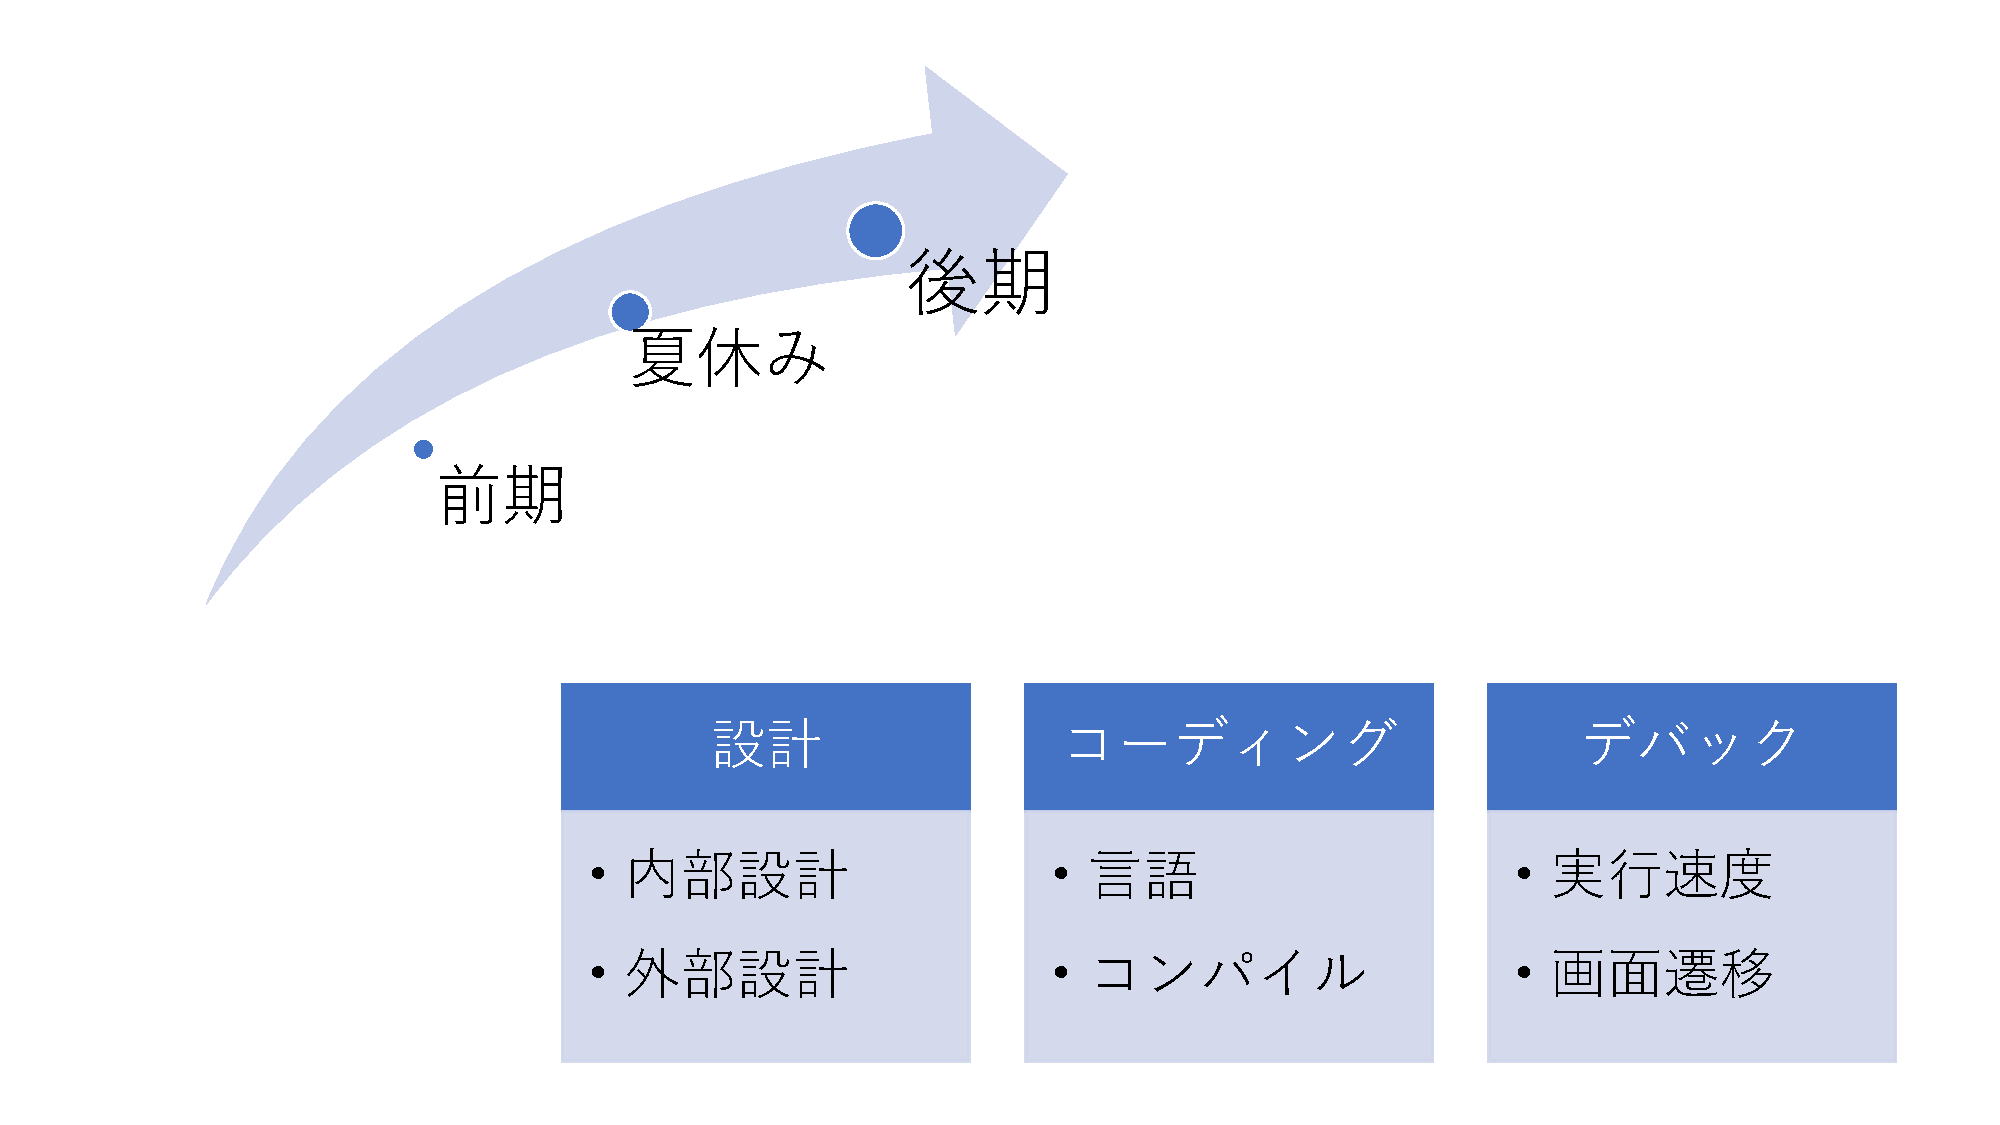
\includegraphics[scale=0.4, clip]{./img/illust.pdf}    
        \caption{図の名前}
        \label{fig:図の名前}
    \end{center}
    \end{screen}
    \end{figure}
    \end{verbatim}

    |表示例:PDF|
    \begin{figure}[!h]
    \begin{screen}
    \begin{center}
        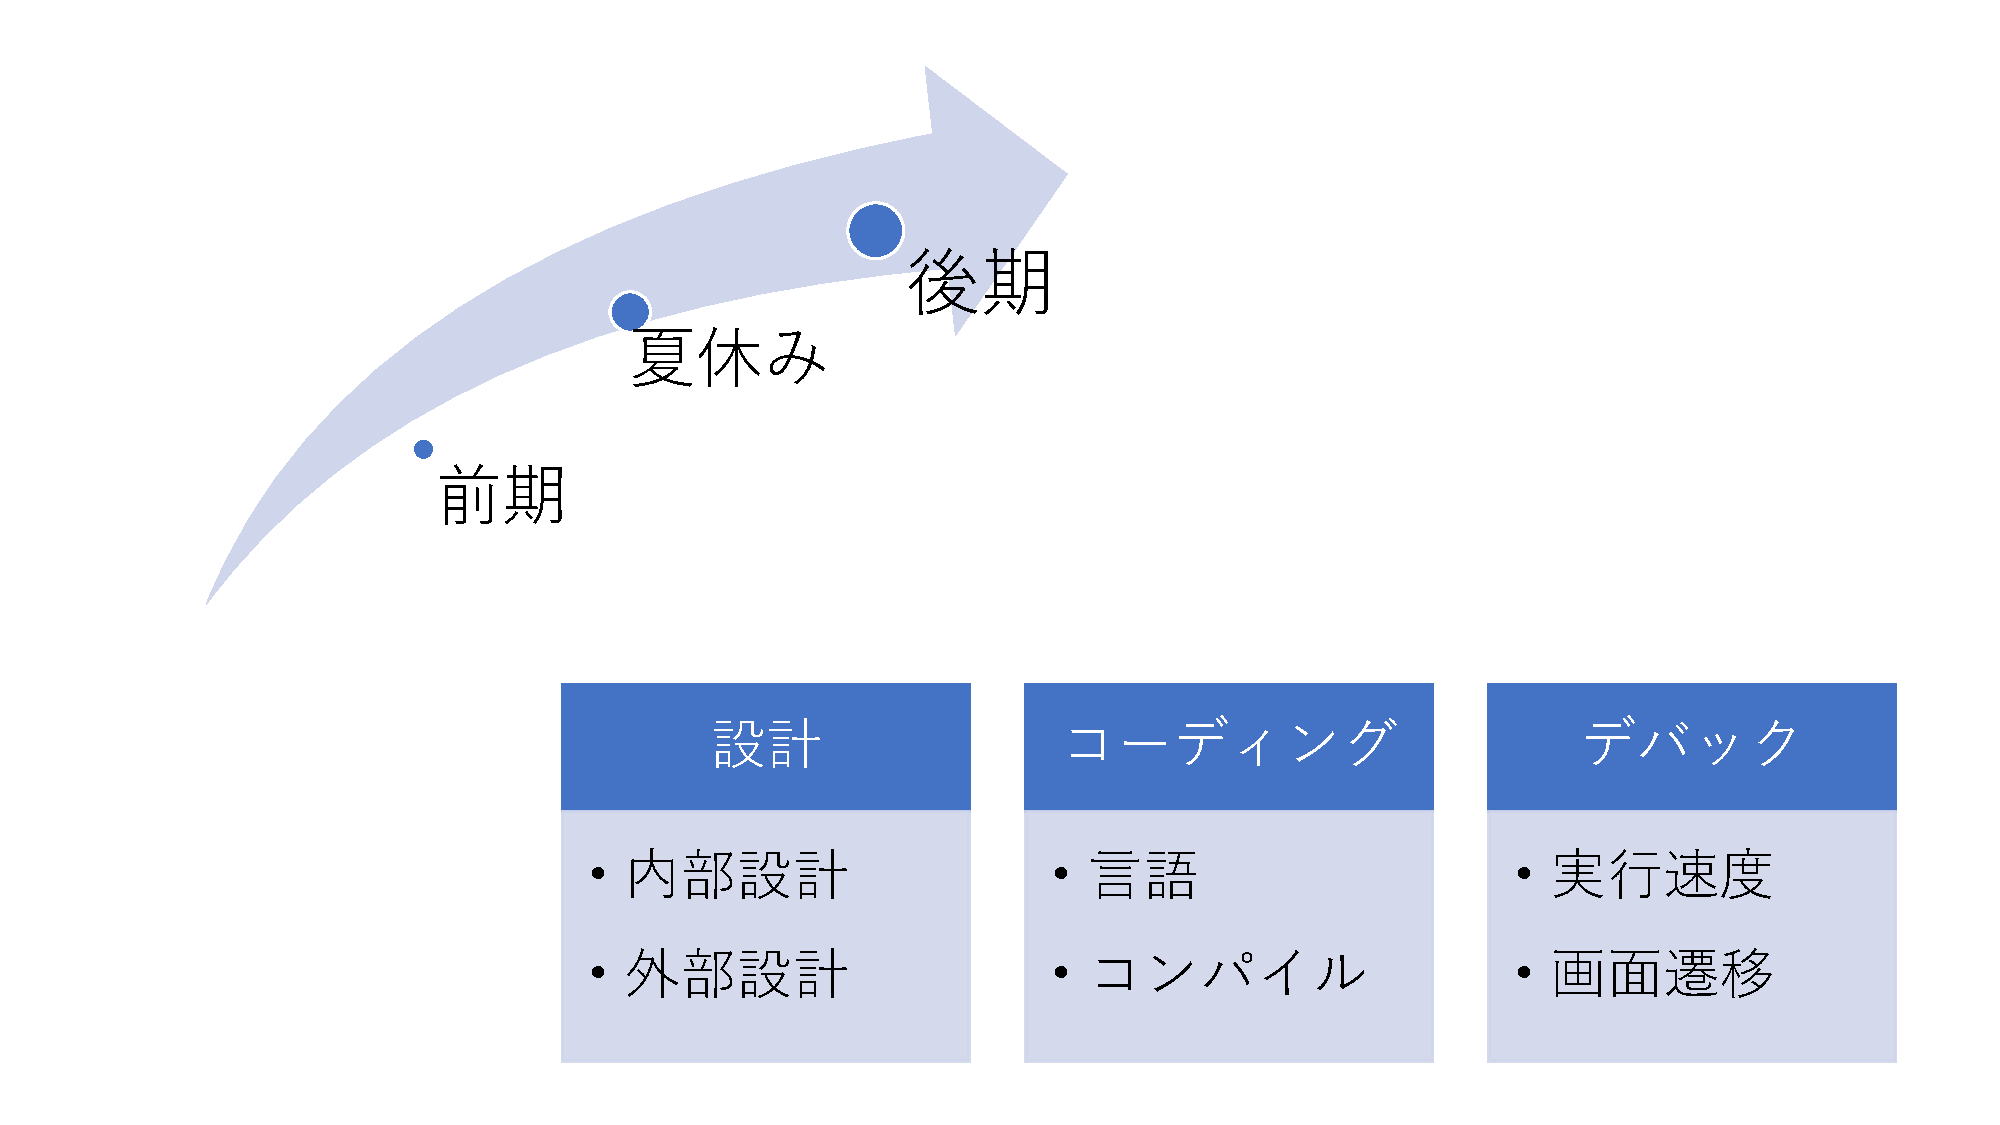
\includegraphics[scale=0.4, clip]{./img/illust.pdf}
        \caption{図の名前}
        \label{fig:図の名前}
    \end{center}
    \end{screen}
    \end{figure}


    \begin{itemize}
        \item figure環境

        図を表示するための場所を作ります.[!h]は「なるべくその場所に表示する」というオプションです.
        \item screen環境

        図を囲むための枠を表示します.
        \item center環境

        囲んだ部分を中央ぞろえで表示します.
        \item includegraphicsコマンド

        図を表示します.\{\}内に表示する図のパスを記述します.[scale=0.4, clip]は「拡大率0.4ではみ出した部分は切り取る」というオプションです.\\
        オプションには「width」「height」「angle」があります.カンマで区切ることで複数指定することが可能です.
	 \item captionコマンド
	
	 図にキャプションをつけます。番号は自動で振られます。
    \end{itemize}
    labelコマンドについては\ref{sec:reference_chapter}を参照してください.

\section{表の表示}
\label{sec:chart_table}
    表を表示する場合,table環境を使用します.一行は\&で区切ります.行端には改行を記述します.\\
    |記述例|
    \begin{verbatim}
    \begin{table}[!h]
    \begin{center}
    \caption{表の名前}
    \label{fig:表の名前}
    \begin{tabular}{|l|c|r||r|}
    \hline
        \multicolumn{2}{|l|}{メニュー} 
            & \multicolumn{1}{c||}{値段} 
                & \multicolumn{1}{p{8zw}|}{カロリー}\\ \hline \hline
             & 並盛 & 500円 & 600 kcal \\ \cline{2-4}
        牛丼 & 大盛 & 1,000円 & 800 kcal \\ \cline{2-4}
             & 特盛 & 1,500円 & 1,000 kcal \\ \hline
             & 並盛 & 300円 & 250 kcal \\ \cline{2-4}
        牛皿 & 大盛 & 700円 & 300 kcal \\ \cline{2-4}
             & 特盛 & 1,000円 & 350 kcal \\ \hline
    \end{tabular}
    \end{center}
    \end{table}
    \end{verbatim}

|表示例|
		\newcolumntype{Y}{>{\centering\arraybackslash}p{10zw}}
    \begin{table}[!h]
    \begin{center}
    \caption{表の名前}
    \label{fig:表の名前}
    \begin{tabular}{|l|c|r||r|}
    \hline
            \multicolumn{2}{|Y|}{メニュー} & \multicolumn{1}{c||}{値段} & \multicolumn{1}{p{8zw}|}{カロリー}\\ \hline \hline
             & 並盛 & 500円 & 600 kcal \\ \cline{2-4}
            牛丼 & 大盛 & 1,000円 & 800 kcal \\ \cline{2-4}
             & 特盛 & 1,500円 & 1,000 kcal \\ \hline
             & 並盛 & 300円 & 250 kcal \\ \cline{2-4}
            牛皿 & 大盛 & 700円 & 300 kcal \\ \cline{2-4}
             & 特盛 & 1,000円 & 350 kcal \\ \hline
    \end{tabular}
    \end{center}
    \end{table}
    \begin{itemize}
    \item table環境

    表を表示するための場所を作ります.
       \item tabular環境

       表を表示します.\{\}内に列の書式を設定しています.\\
    l:左寄せ c:センタリング r:右寄せ |:縦罫線\\
    表内に文章を入れる場合や,カラム幅を指定したい場合は列書式に「\verb|p{5cm}|」のように記述します.カラム幅を指定しない場合は自動で幅が設定されます.
    \item hlineコマンド

    横罫線を表示します.
    \item clineコマンド

    特殊横罫線を表示します.\{\}内に線を引きたいカラムを指定します.上記では2~4カラムを指定しています.
    \item multicolumnコマンド

    カラムを結合します.\verb|\multicolumn{結合カラム数}{書式}{文字列}|
    \end{itemize}



\chapter{論文内の参照}
\label{chp:reference}

\section{脚注}
\label{sec:reference_ftnote}
	文章中に脚注を使用したい場合はfootnoteコマンドを使用します.「\verb|\footnote[番号]{内容}|」のように記述します\footnote[99]{脚注表示例.}.番号を省略した場合には自動で番号が振られます\footnote{番号省略例}.

\section{引用}
\label{sec:reference_quote}
	文献等の引用を行う場合には,quote環境またはquotation環境を使用します.\\
	|quote表示例|
	\begin{quote}
		quoteは短文の引用に用いられます.

		quoteは段落の先頭字下げを行いません.
	\end{quote}
	|quotation表示例|
	\begin{quotation}
		quotationは長文の引用に用いられます.quotationは段落の先頭字下げを行います.

		quote環境とquotation環境では環境外の文章から一段下がって表示されています.
	\end{quotation}

\section{参考文献}
\label{sec:reference_bib}
	参考文献があることを示したい場合はciteコマンドを使用します.「\verb|\cite{参考文献}|」のように記述します\cite{Webデザイン}.

	参考文献一覧は巻末に記載しています.citeコマンドの引数にはthebibliography環境内のbibitemコマンドに記載した名前を使用することで,番号が表示されます.thebibliography環境の引数は参考文献の最大数で,配列を宣言する場合と同じ考えです.特に理由がなければ99のままでよいでしょう.

\section{章節番号・図表番号}
\label{sec:reference_chapter}
	章節や図表の番号を参照する場合にはlabelコマンドとrefコマンドを使用します.事前に章節等を記述している部分にlabelコマンドで名前をつけ,呼び出す際にその名前をrefコマンドで使用することで番号を表示することができます.

	呼び出すことのできるのは番号のみのため,前後に言葉を補う必要があります.\\
	|記述例|
	\begin{verbatim}
		\chapter{論文内の参照}
		\label{chp:reference}

		この部分については第\ref{chp:reference}章を参照してください.
	\end{verbatim}
	|表示例|\
		この部分については第\ref{chp:tex_basic}章(第2章の参照名を確認)参照してください.
	

\chapter{Texの書き方(応用編)}
\label{chp:tex_pro}

\section{応用コマンド・環境}
\label{sec:tex_pro_cmd}
\subsection{newcolumntypeコマンド}
\label{sub:tex_pro_cmd_newcol}
	表のカラムの書式を新規に割り当てることのできるコマンドです。表を作成する前に当コマンドで新しい書式を作成することで使用することが可能です。\\
	「\verb|\newcolumntype{書式名}{書式}|]」のように記述することで書式を作成することができます。
幅が5cmで中央ぞろえのカラムを作成する場合には\\「\verb|>{\centering\arraybackslash}p{5cm}|」を書式に記載します。

\subsection{breakbox環境}
\label{sub:tex_pro_cmd_break}
	枠で囲まれた文章を作成することができます。図を囲むscreen環境と違い、ページをまたいだ枠を作ることができます。ソースコードを載せる場合等に使用するとよいでしょう。\\
	|表示例|
\begin{breakbox}
\noindent breakbox環境内の文章です。breakbox環境内の文章です。breakbox環境内の文章です。breakbox環境内の文章です。breakbox環境内の文章です。breakbox環境内の文章です。breakbox環境内の文章です。breakbox環境内の文章です。breakbox環境内の文章です。breakbox環境内の文章です。breakbox環境内の文章です。breakbox環境内の文章です。breakbox環境内の文章です。breakbox環境内の文章です。
\end{breakbox}

\section{マクロ}
\label{sec:tex_pro_macro}
	Latexのマクロはコマンドと環境の両方を作成することが可能です。

\subsection{コマンドマクロ}
\label{sub:tex_pro_macro_cmd}
	コマンドのマクロは「\verb|\newcommand{コマンド名}{内容}|」のように記述することで作成することができます。引数を指定することもでき、「\verb|\newcommand{コマンド名}[引数の数]{(#1)内容}|」のように記述します。\\
	|記述例|
	\begin{verbatim}
		\newcommand{\hoge}[2]{#1 は #2 である}
		作成したコマンドを使用する場合は「\hoge{我輩}{猫}」のように記述します。
	\end{verbatim}
	|表示例|\\
	\newcommand{\hoge}[2]{#1 は #2 である}
	作成したコマンドを使用する場合は「\hoge{我輩}{猫}」のように記述します。

\subsection{環境マクロ}
\label{sub:tex_pro_macro_env}
    環境のマクロは「\verb|\newenvironment{環境}[引数の数]{はじめ}{おわり}|」のように記述することで作成することができます。コマンドと同じく引数を指定できます。\\
	|記述例|
	\begin{verbatim}
	\newenvironment{fig}{
	    \begin{figure}[!h]
	    \begin{screen}
	    \begin{center}
	}{
	    \end{center}
	    \end{screen}
	    \end{figure}
	}
	\begin{fig}
	    
\includegraphics[scale=0.4, clip]{./img/apple.png}
	    \caption{図の名前}
	    \label{fig:図の名前}
	\end{fig}
	\end{verbatim}
	|表示例|
	\newenvironment{fig}{
	    \begin{figure}[!h]
	    \begin{screen}
	    \begin{center}
	}{
	    \end{center}
	    \end{screen}
	    \end{figure}
	}
	\begin{fig}
	    
\includegraphics[scale=0.4, clip]{./img/apple.png}
	    \caption{図の名前}
	    \label{fig:図の名前}
	\end{fig}

\newpage

%%%%%%%本文 end%%%%%%%%%%%%%%%%%%%%%%%%%%%%%%%%%%%%%%%%%%%%

%%%%%%%謝辞 start%%%%%%%%%%%%%%%%%%%%%%%%%%%%%%%%%%%%%%%%%%%

\chapter*{ \\謝辞}\addcontentsline{toc}{chapter}{謝辞}
|記述例|

本研究に関しまして,熱心かつ丁寧にご指導いただきました,
千葉工業大学情報科学研究科情報科学専攻中村直人教授に心から御礼申し上げます.
また,修士論文発表における,副査を務めていただきました浮貝雅裕教授,須田宇宙准教授に深謝いたします.
そして,中村研究室博士前期課程,学部生の皆様,および,卒業された博士前期課程,学部生の皆様に心から御礼申し上げます.
皆様のおかげで,これまでの研究生活を充実かつ楽しく送ることが出来ました.
そして,これまで支えてくれた両親をはじめとする親族各位に改めて御礼申し上げます.
ありがとうございました.

%%%%%%%謝辞 end%%%%%%%%%%%%%%%%%%%%%%%%%%%%%%%%%%%%%%%%%%%%

%%%%%%%参考文献 start%%%%%%%%%%%%%%%%%%%%%%%%%%%%%%%%%%%%%%%%%%%
\begin{thebibliography}{99}\addcontentsline{toc}{chapter}{参考文献}

\bibitem{Webデザイン}
Webデザイン編集委員会,“Webデザイン-コンセプトメイキングから運用まで- 改訂版”,CG-ARTS協会(2013).

\bibitem{数値計算法}
三井田惇郎/須田宇宙,“数値計算法 第2版”,森北出版株式会社(2013).


\end{thebibliography}
%%%%%%%参考文献 end%%%%%%%%%%%%%%%%%%%%%%%%%%%%%%%%%%%%%%%%%%%
\end{document}

%%%%%%%コンテンツ end%%%%%%%%%%%%%%%%%%%%%%%%%%%%%%%%%%%%%%%%%%%%